\documentclass{article}
\usepackage{graphicx} % Required for inserting images
\usepackage [utf8]{ctex}
\usepackage{listings}
\usepackage{geometry}

\title{News-Category-Classification}
\author{211870287 丁旭 }
\date{November 2023}

\geometry{left = 1cm}
\begin{document}
% \maketitle

\section{数据集描述(包括统计数据、图表等)}
\section{读取数据}
\begin{lstlisting}
# 读取JSON文件并合并为列表
data = []
with open('News_Category.json', 'r') as file:
    for line in file:
        data.append(json.loads(line))

# 将JSON数据转换为DataFrame
df = pd.DataFrame(data)
\end{lstlisting}


\section{数据集描述(包括统计数据、图表等)}
\subsection{类别数目及占比统计}
\begin{lstlisting}
category_counts = df['category'].value_counts()
    # 绘制饼图
    plt.figure(figsize=(8, 6))
    plt.pie(category_counts, labels=category_counts.index, autopct='%1.1f%%')
    plt.title('Category Distribution')
    plt.axis('equal')

    # 显示图形
    plt.show()
\end{lstlisting}
\begin{lstlisting}
# 绘制柱状图
    plt.figure(figsize=(10, 6))
    plt.bar(category_counts.index, category_counts)
    plt.xlabel('Category')
    plt.ylabel('Count')
    plt.title('Category Distribution')

    # 自动调整x轴标签的旋转角度
    plt.xticks(rotation=90)

    # 显示图形
    plt.show()
\end{lstlisting}
\begin{center}
    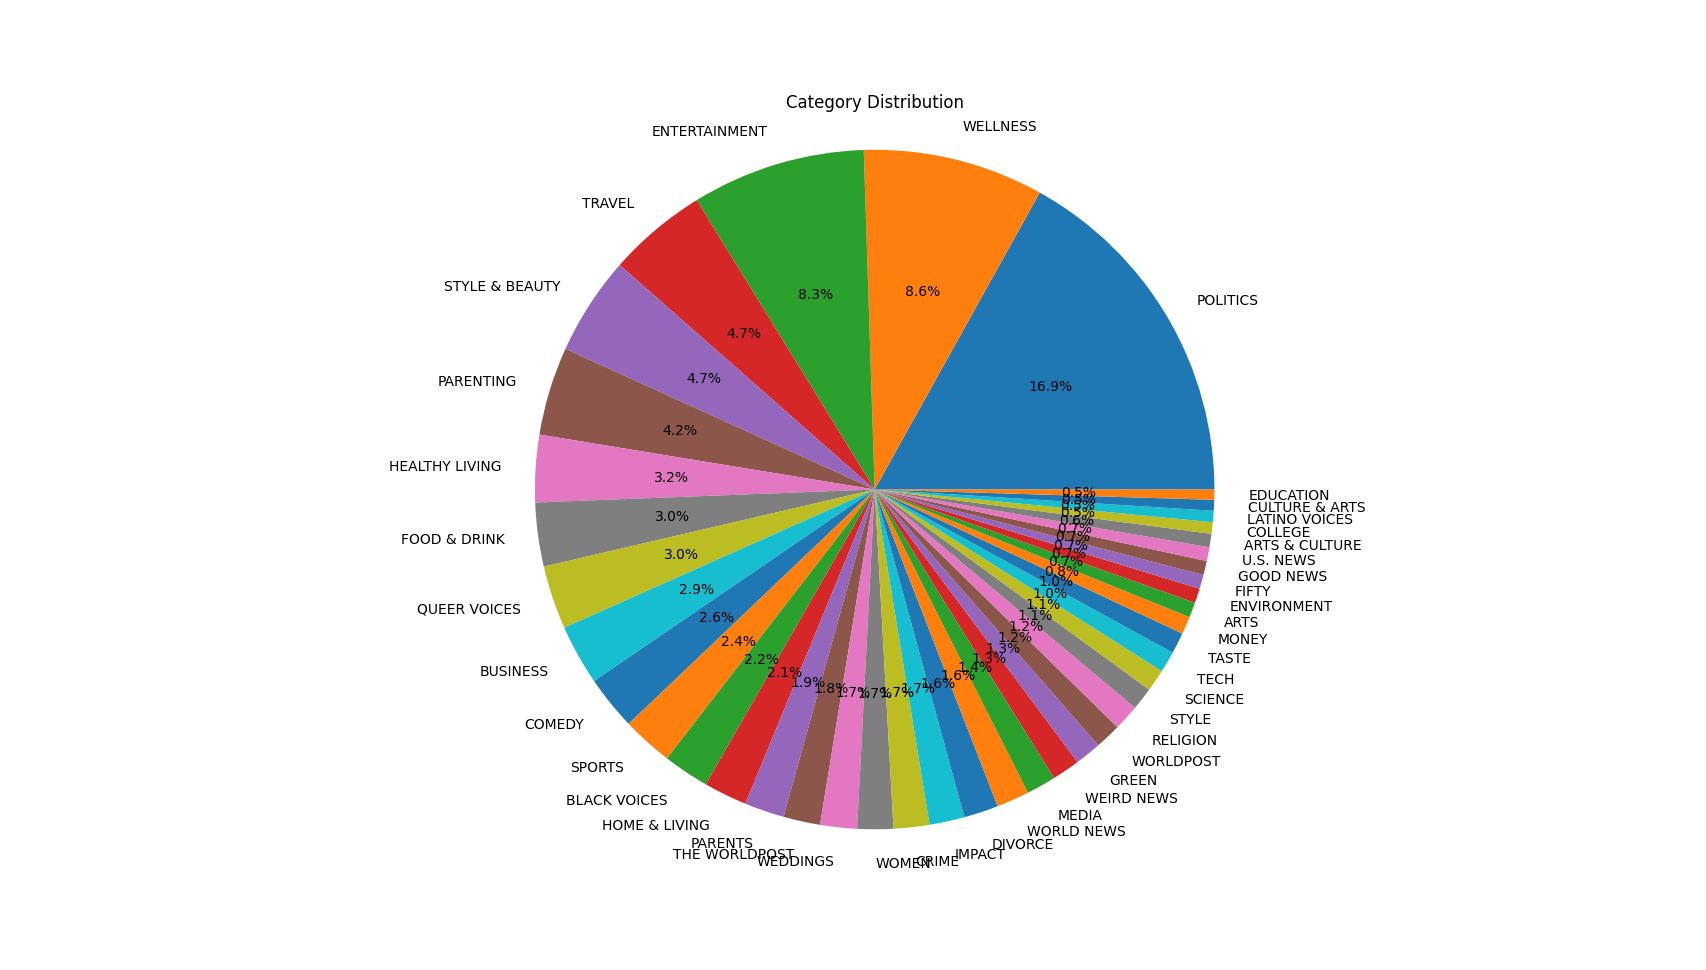
\includegraphics[width=1\linewidth]{分类.png}
\end{center}
\begin{center}
    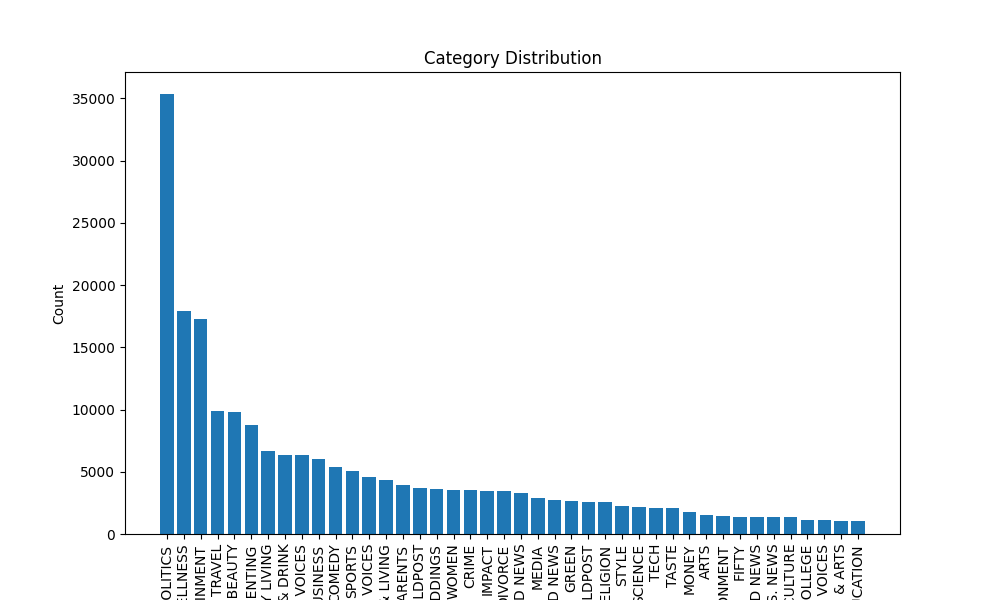
\includegraphics[width=1\linewidth]{类别柱状图.png}
\end{center}
\subsection{新闻词频统计}
\begin{lstlisting}
def most_common_words():

    nltk.download('stopwords')

    stop_words = set(stopwords.words('english'))
    tokenizer = nltk.RegexpTokenizer(r'\w+')

    content = ''.join(df['short_description']) + ''.join(df['headline'])
    tokens = tokenizer.tokenize(content.lower())
    filtered_tokens = [token for token in tokens if token not in stop_words]

    word_count = Counter(filtered_tokens)
    top_100 = word_count.most_common(100)
    # 创建词云对象并生成词云图
    wordcloud = WordCloud(width=800, height=400, background_color='white').generate_from_frequencies(dict(top_100))

    # 显示词云图
    plt.figure(figsize=(10, 5))
    plt.imshow(wordcloud, interpolation='bilinear')
    plt.axis('off')
    plt.show()
\end{lstlisting}

\begin{center}
    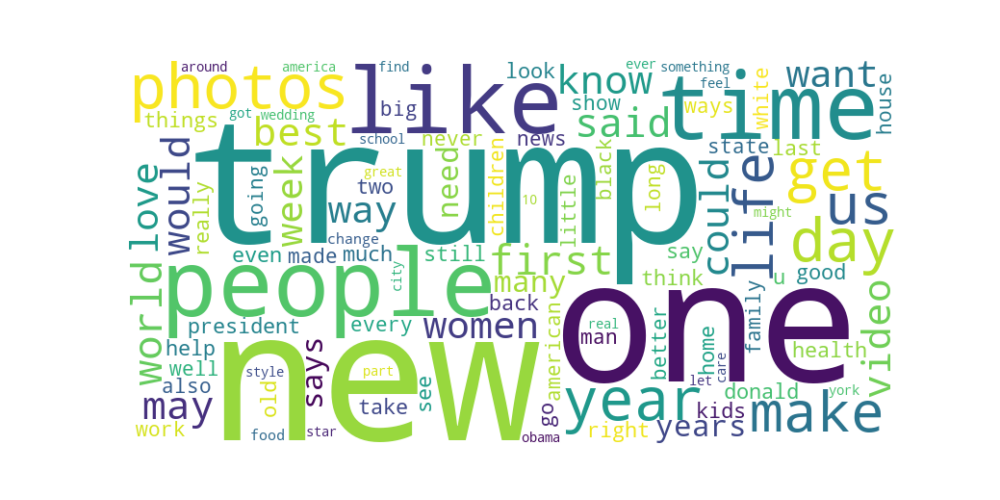
\includegraphics[width=1\linewidth]{词云.png}
\end{center}
\begin{center}
    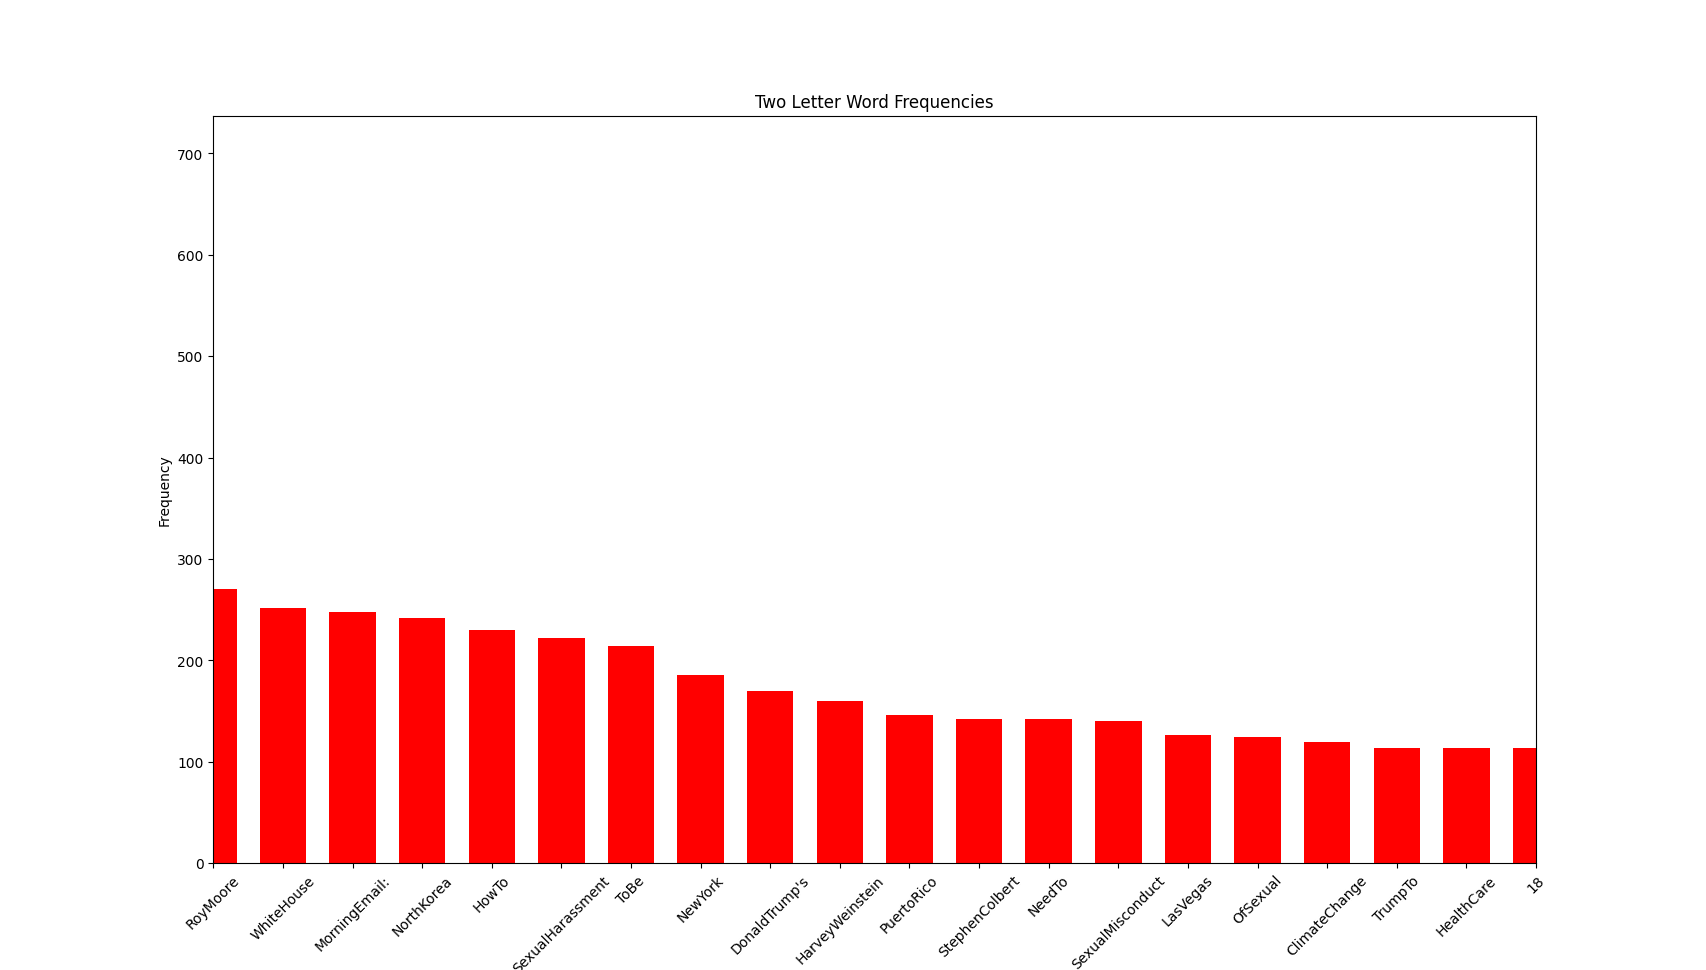
\includegraphics[width=1\linewidth]{词组的词频.png}
\end{center}


\newpage
\section{ 数据处理的流程}
\subsection{合并headline和short-description作为模型的输入数据}
\begin{lstlisting}
df['text'] = df.headline + " " + df.short_description
\end{lstlisting}
\subsection{对文本进行清洗,包括将文本转换为小写、去除特殊字符等操作}
\begin{lstlisting}
def clean_str(string):
    string = re.sub(r"[^A-Za-z0-9(),!?\'\`]", " ", string)
    return string.lower()

df['text'] = df['text'].apply(clean_str)
\end{lstlisting}
\subsection{将文本转化为TF-IDF特征向量}
\begin{lstlisting}
import re, string
re_tok = re.compile(f'([{string.punctuation}“”¨«»®´·º½¾¿¡§£₤‘’])')
def tokenize(s): return re_tok.sub(r' \1 ', s).split()

tfidf_converter = TfidfVectorizer(min_df=3, max_df=0.9, strip_accents='unicode',tokenizer=tokenize,ngram_range=(1,2),sublinear_tf=1)
X_train_tfidf = tfidf_converter.fit_transform(X_train)
X_test_tfidf = tfidf_converter.transform(X_test)
\end{lstlisting}
\subsection{划分训练集和测试集}
\begin{lstlisting}
X_train, X_test, y_train, y_test = train_test_split(df['fulltext_processed'], df['category'], test_size=0.2, random_state=0)
\end{lstlisting}


\section{分类模型选择及设计、训练、验证、测试}
\subsection{朴素贝叶斯分类器进行训练和测试}
\begin{lstlisting}
# 使用CountVectorizer将文本转换为词频向量表示
vectorizer = CountVectorizer()
X_train_counts = vectorizer.fit_transform(X_train)
X_test_counts = vectorizer.transform(X_test)

# 初始化MultinomialNB分类器
classifier = MultinomialNB()

# 在训练集上训练分类器
classifier.fit(X_train_counts, y_train)

# 在测试集上进行预测
y_pred = classifier.predict(X_test_counts)

# 计算准确率
accuracy = accuracy_score(y_test, y_pred)

# 计算混淆矩阵
confusion_mat = confusion_matrix(y_test, y_pred)

# 输出分类报告
classification_rep = classification_report(y_test, y_pred)

# 打印结果
print("Accuracy:", accuracy)
print("Confusion Matrix:\n", confusion_mat)
print("Classification Report:\n", classification_rep)
\end{lstlisting}
\begin{center}
    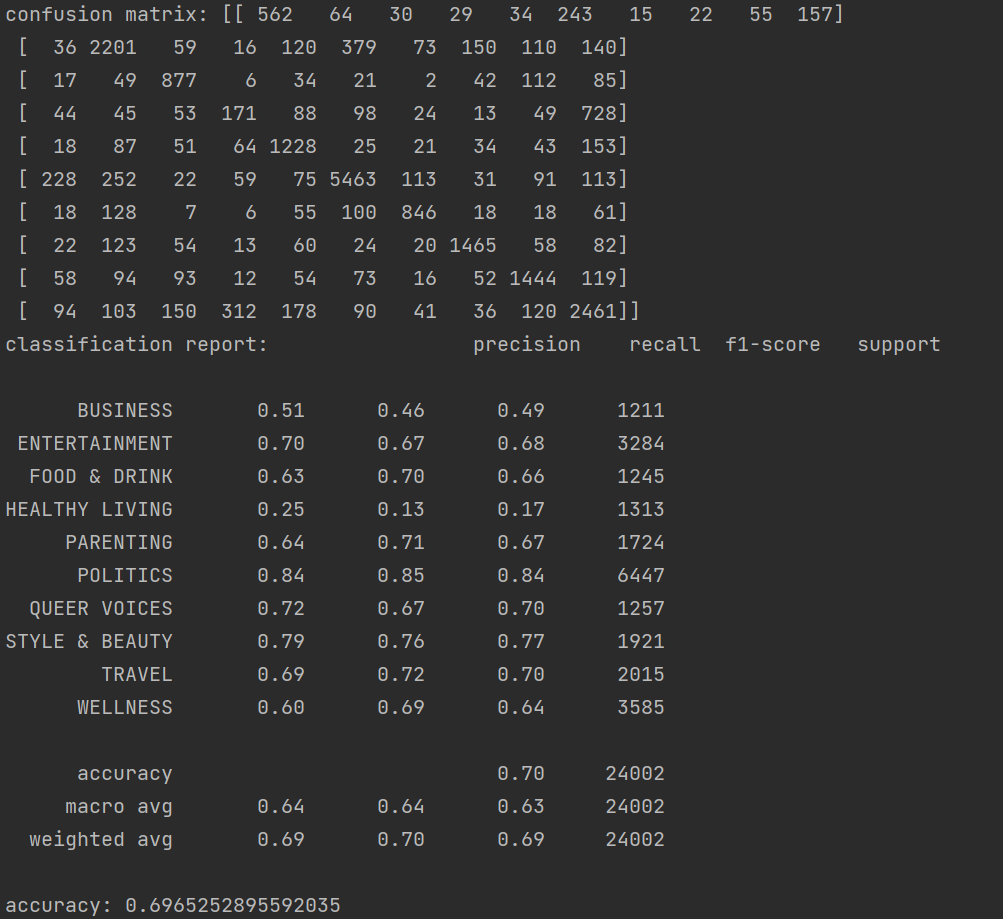
\includegraphics[width=1\linewidth]{1.png}
\end{center}
\subsection{支持向量机(SVM)进行训练和测试}
\begin{lstlisting}
# 使用TfidfVectorizer将文本转换为TF-IDF向量表示
vectorizer = TfidfVectorizer()
X_train_tfidf = vectorizer.fit_transform(X_train)
X_test_tfidf = vectorizer.transform(X_test)

# 初始化LinearSVC分类器
classifier = LinearSVC()

# 在训练集上训练分类器
classifier.fit(X_train_tfidf, y_train)

# 在测试集上进行预测
y_pred = classifier.predict(X_test_tfidf)

# 计算准确率
accuracy = accuracy_score(y_test, y_pred)

# 计算混淆矩阵
confusion_mat = confusion_matrix(y_test, y_pred)

# 输出分类报告
classification_rep = classification_report(y_test, y_pred)

# 打印结果
print("Accuracy:", accuracy)
print("Confusion Matrix:\n", confusion_mat)
print("Classification Report:\n", classification_rep)
\end{lstlisting}
\begin{center}
    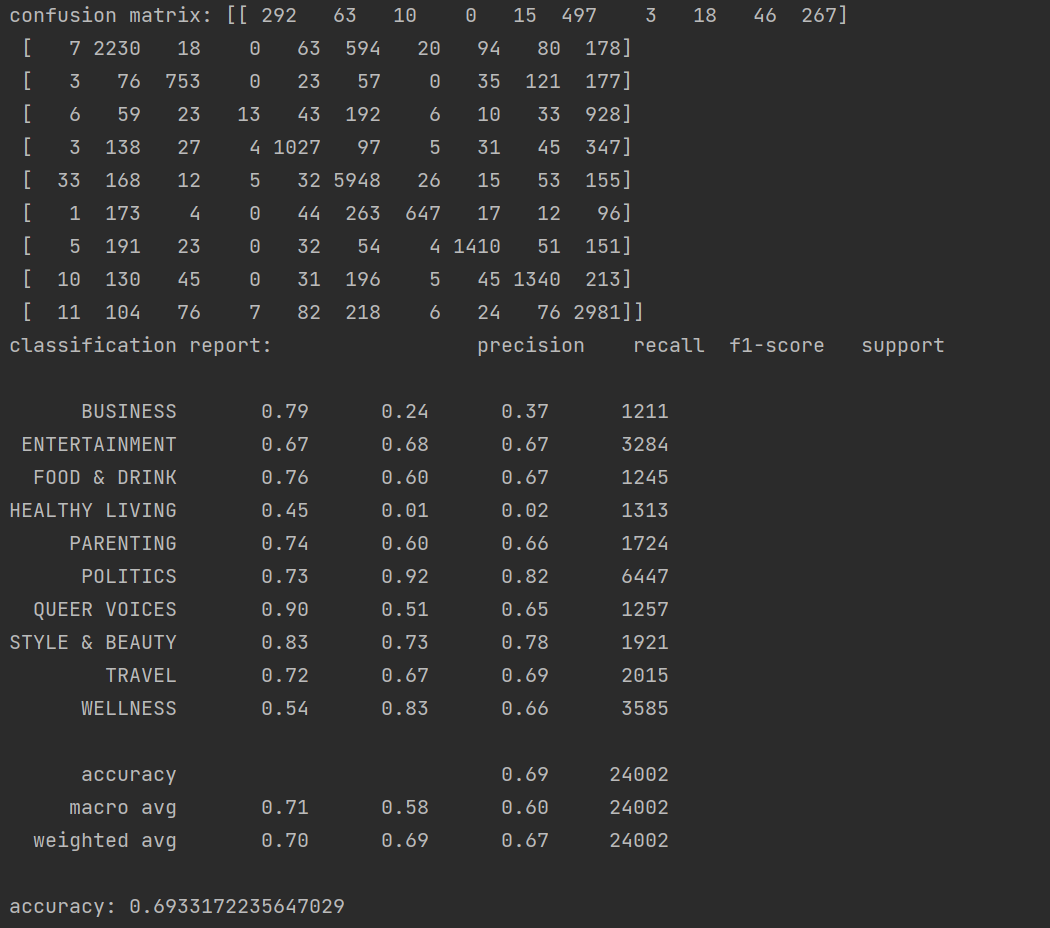
\includegraphics[width=1\linewidth]{2.png}
\end{center}
\subsection{逻辑回归进行训练和测试}
\begin{lstlisting}
# 使用TfidfVectorizer将文本转换为TF-IDF向量表示
vectorizer = TfidfVectorizer()
X_train_tfidf = vectorizer.fit_transform(X_train)
X_test_tfidf = vectorizer.transform(X_test)

# 初始化LogisticRegression分类器
classifier = LogisticRegression()

# 在训练集上训练分类器
classifier.fit(X_train_tfidf, y_train)

# 在测试集上进行预测
y_pred = classifier.predict(X_test_tfidf)

# 计算准确率
accuracy = accuracy_score(y_test, y_pred)

# 计算混淆矩阵
confusion_mat = confusion_matrix(y_test, y_pred)

# 输出分类报告
classification_rep = classification_report(y_test, y_pred)

# 打印结果
print("Accuracy:", accuracy)
print("Confusion Matrix:\n", confusion_mat)
print("Classification Report:\n", classification_rep)
\end{lstlisting}
\begin{center}
    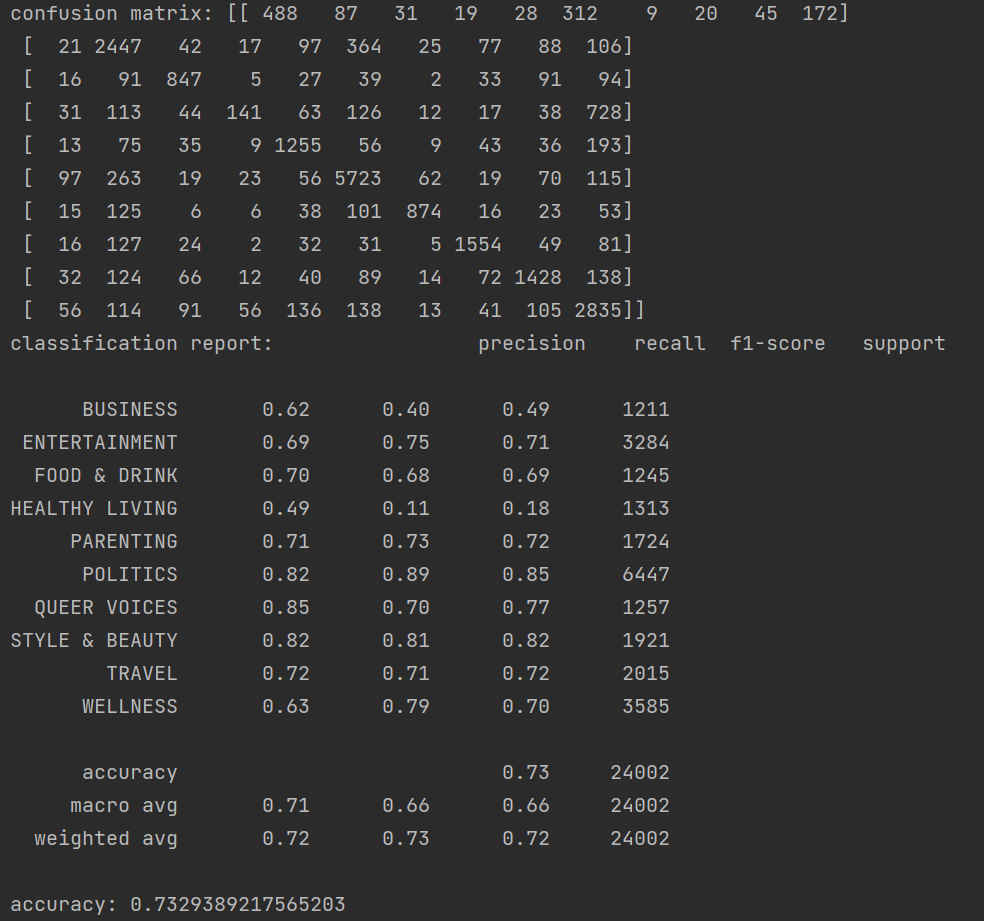
\includegraphics[width=1\linewidth]{3.png}
\end{center}
\subsection{对文本进行词干化和词形还原及效果验证}
有将近百分之90的正确率
\begin{lstlisting}
from nltk.stem import PorterStemmer, WordNetLemmatizer
stop_words = set(stopwords.words('english'))
def stem_text(rawsentence):
    stemmer = PorterStemmer()
    tokens = word_tokenize(rawsentence)
    stemmed_tokens = [stemmer.stem(word) for word in tokens if word not in stop_words]
    return stemmed_tokens

tfidf_converter = TfidfVectorizer(max_features=1500,min_df=5,max_df=0.7, stop_words=None,tokenizer=stem_text)
X_train_tfidf = tfidf_converter.fit_transform(X_train)
X_test_tfidf = tfidf_converter.transform(X_test) 

print(tfidf_converter.get_feature_names())

classifier = MultinomialNB().fit(X_train_tfidf, y_train)
y_pred = classifier.predict(X_test_tfidf)
print('confusion matrix:',confusion_matrix(y_test,y_pred))
print('classification report:', classification_report(y_test,y_pred))
print('accuracy:',accuracy_score(y_test, y_pred))
\end{lstlisting}
\begin{center}
    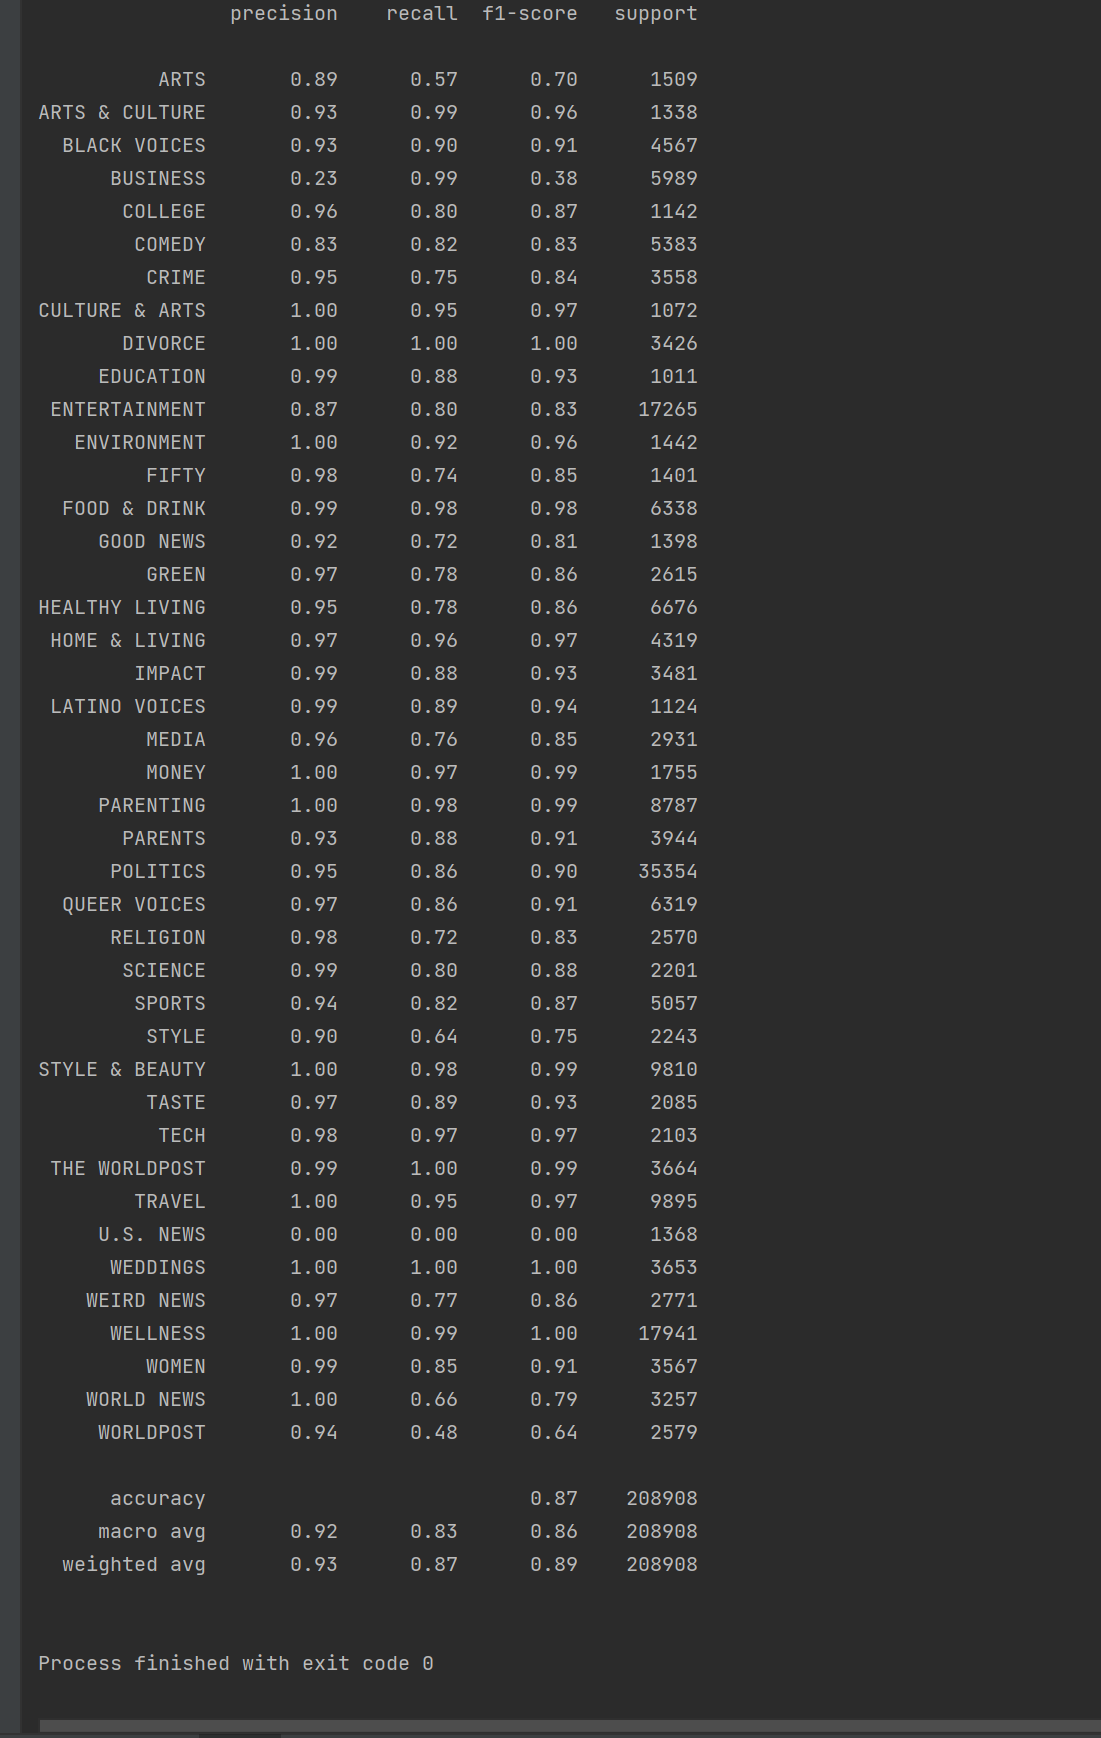
\includegraphics[width=1\linewidth]{4.png}
\end{center}
\section{最终选定knn模型}
\subsection{模型的正确率}
模型的正确率为百分之88
\begin{center}
    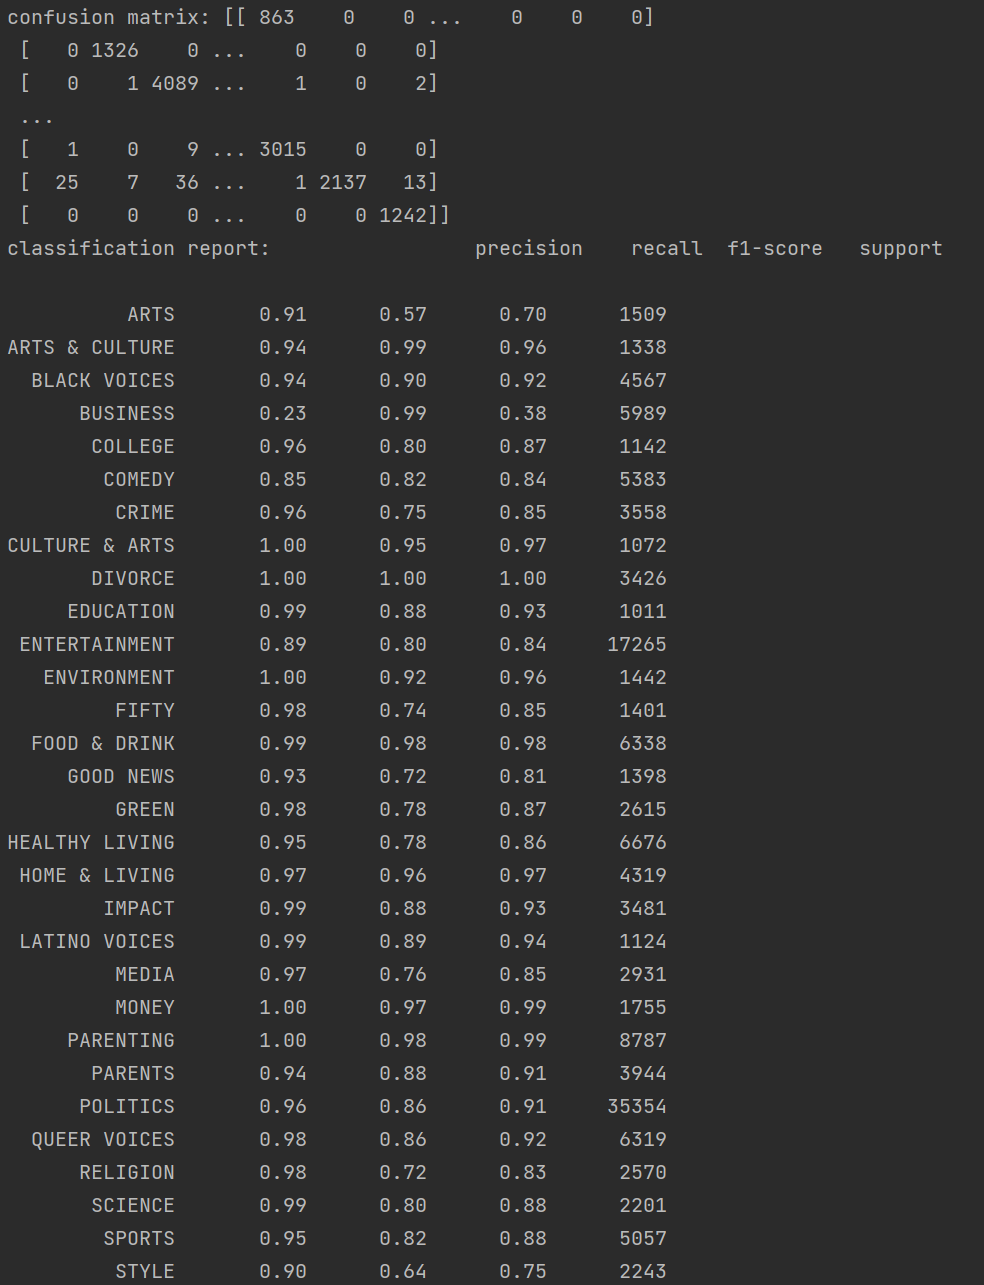
\includegraphics[width=1\linewidth]{5.png}
\end{center}
\begin{center}
    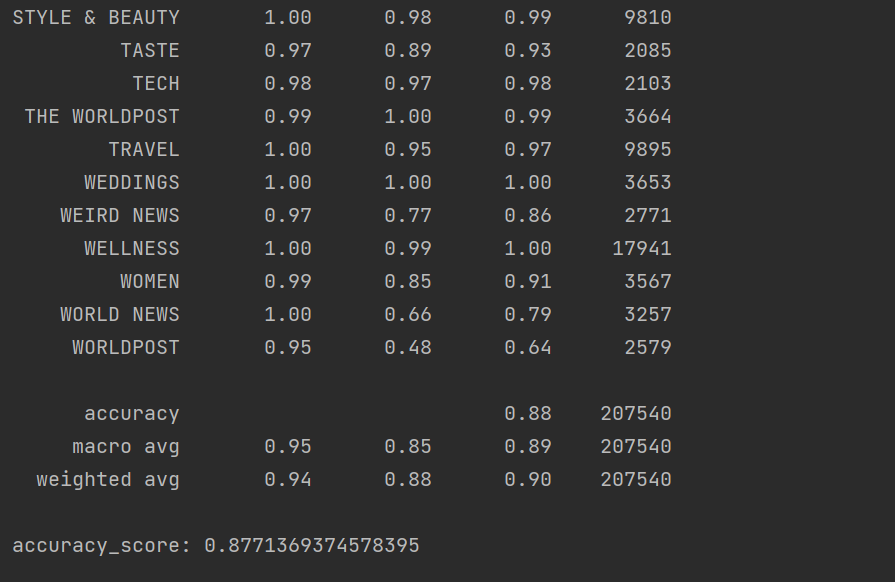
\includegraphics[width=1\linewidth]{6.png}
\end{center}
\subsection{模型的调用方法}

\begin{lstlisting}
#参数为json文件的路径
def predict_json(pathToJson):
    df = load_test_set(pathToJson)
    df['short_description'] = df.short_description.apply(process_text)
    df['short_description'] = df.short_description.apply(join_word)
    knn, vec = joblib.load('knn_model.joblib')

    feature = vec.transform(df['short_description'])

    prediction = knn.predict(feature)

    print('confusion matrix:', confusion_matrix(df['category'], prediction))

    print('classification report:', classification_report(df['category'], prediction))

    print('accuracy_score:', accuracy_score(df['category'], prediction))

#参数为新闻的headline, authors, link, des, date
def predict(headline, authors, link, des, date):
    model, vec = joblib.load('knn_model.joblib')
    feature = vec.transform([des])
    prediction = model.predict(feature)
    print(prediction[0])
\end{lstlisting}

\end{document}
